\documentclass[a4paper,10pt]{scrartcl}
\usepackage[utf8]{inputenc}
\usepackage{graphicx}
\usepackage{float}

% Title Page
\title{Codmon: A multi-platform modular test environment.}
\author{Berend van Veenendaal}
\bibliographystyle{plain}
%hieronder wordt de project naam als variabele gedeclareerd
\newcommand{\project}{Codmon 2.0}
\newcommand{\CS}{C\nolinebreak\hspace{-.05em}\raisebox{.6ex}{\bf \#}}

\begin{document}
\maketitle

\begin{abstract}
TODO:Abstract
\end{abstract}
\newpage
\section*{Preface}
\label{sec:Preface}
TODO: Preface,acknowledgements
\newpage
\tableofcontents
\newpage

\section{Introduction}
\label{sec:Introduction}
This chapter introduces the \project{} project by giving a brief description of background of my research and of the
previous version of the Codmon project. It also describes the structure of this thesis.

\subsection{Background}
\label{sec:Background}
In times when software projects become more and more complex, testing of this software becomes more and more important. Many software related problems are caused by lack of testing of the 
software~\cite{TTCST}. Most of the times software testers only test software on one platform. For instance only on a Linux or a Windows platform. Setting-up and configuring again and again all 
the different test environments on different platforms simply costs too much time. So one of the challenges of software testing is to make sure that the software behaves in the same way on 
different platforms, without spending to much time on the installation and configuration of the test environment on all these platforms. Even when the test environment is written in such a way 
that it is able to run on different platforms, there are still issues that must be dealt with, before one is able to run and test the software. So in an ideal world we can test the software without being 
worried about setting up the test environment. 

\subsection{Problem indication}
\label{subsec:Problemindication}
Nowdays there are numerous test frameworks and test environments available. For example there is \emph{Junit}\cite{Junit} for Java-unit testing and \emph{NUnit}\cite{Nunit} for \CS{}-unit testing.
There are also different environments like Hudson\cite{HudsonDoc}\cite{Hudson}, Jenkins\cite{JenkinsDoc} which can build a project and run a series of (unit) tests against this project. 
These frameworks and environments have both their advantages and disadvantages. One of the advantages of unit testing is that a software developer can easily add new \emph{functional} unit tests.
One of the disadvantages is that standard unit testing ignores non-functional tests like performance testing and the deployment of the software. Jenkins and Hudson,like Unit tests, also have their
disadvantages. For instance, although they both run on several platforms, in their usage they are not really platform independent. For example, if you want
to make a connection from Hudson or Jenkins to a remote machine you do this by executing a shell script, so a user must know in advance on which platform this script has to run.
So although it is possible to connect to different machines it is not a 100\% platform independent environment.
 
\subsection{Problem statement}
\label{subsec:Problemstatement}
The test frameworks and test environments mentioned in section \ref{subsec:Problemindication} can be criticized on one or more aspects. What we are looking for is in fact, a combination
of the positive aspects of the described frameworks and environments, without the undesirable aspects. So the central question is, is it possible to design a
multi-platform, modular test environment? In addition, we study if it is possible to design the test environment in a \emph{user friendly} way, meaning that it must
be possible to easily add both new test cases and software without knowing anything about the internal mechanisms of the test environment.\\

\noindent This thesis describes a multi-platform, user friendly modular test environment called \project{}. The \project{} project provides users with a set of virtual machines,
in which \project{} is already installed and preconfigured. The purpose of the virtual machines is to make it easy for users to test software in several environments. By doing it this way the only tasks
a \project{} user has to do are 1) add their project  to the init.XML file. and 2) add the tests to a so called wrapper file. This will be discussed in more detail in 
section \ref{sec:Codmon2.0}.


\subsection{Thesis outline}
\label{subsec:Thesisoutline}
Section \ref{sec:codmon} first describes the original Codmon framework and why it was built. It also identifies the problems it has. In section \ref{sec:road}, \emph{The road to \project{}}, 
we explain the ideas that came into mind and how we got to the final \project{} design. Section \ref{sec:Codmon2.0} describes the implementation of the \project{} project. 
It starts with a general description of the project followed by a detailed explanation of the different modules of \project{}. After this we will evaluate the choices and the consequences of these 
choices in section \ref{sec:evaluation}. In Section \ref{sec:conclusion} we discuss the results based on section \ref{sec:evaluation}. We end this section with a brief discussion of related work.

\newpage

\section{Codmon}
\label{sec:codmon}
In this section we describe the original Codmon framework and its shortcomings. The original Codmon framework was built in 2005 by François Lesuer\cite{Codmon}. Originally Codmon was built for 
testing and performance monitoring Ibis projects\cite{Ibis}\cite{Satin}\cite{MPJ}\cite{IPL}\cite{GMI} on the DAS-2\cite{das2} computer. Codmon was (At this moment the das2 and Codmon aren't in use anymore.) 
able to perform both functional and performance tests. If for some reason a particular test failed, Codmon reported the problems. It does this by sending an email directly to the programmer who made the last changes 
in code under test. Codmon also reported in the same way in case the performance drops below a certain treshold. The It was also the intention that Codmon would be extensible. In this the Codmon programmers succeeded 
only partially. We will discuss this more in depth in section \ref{subsec:CodmonProblems}.  

\subsection{Codmon Design}
\label{subsec:CodmonDesign}
In this section we will describe the design of the Codmon framework. The setup of Codmon is more or less modular and consists of a few core elements. The set of tests that should run is described
in different configuration files which are called \emph{Sensors}. A sensor describes precisely which tests should be executed and also the software that is under these tests. A sensor consists of two
parts. First there is the \emph{onoff} part, which is used for compilation parts and the functional tests. The core of each sensor element in a sensor file consists of two parts: a wrapper and
a shell-script command. Second there is the \emph{graph} part. This part is used for the performance tests. The results of a performance test will be compared with the results of previous tests 
and if the performance result of a test drops below a certain treshold, an alarm is raised. When an alarm is raised, an email is sent to the last contributor of the code of which a test fails. 
The same happens when one or more functional tests are failing.\\

\noindent Where a \emph{sensor} describes the structure of a set of tests, a so called \emph{wrapper} describes the actual test. Wrappers are small programs that are written int the PERL
language. The return value of a wrapper indicates if a test was successful or not. In case of a failure an alarm is raised and both the return value and the actual error code will be mailed to
the programmer who made the last contribution to the code. The results of the performance tests are plotted in a graph, which makes it easy for the developers to see the performance
behavior. Figure 1 shows a schematic picture of the Codmon structure. More technical details about the Codmon implementation can be found in \cite{Codmon}

\begin{figure}[!ht]
  \caption{\emph{figure 1: Codmon}}
  \centering
    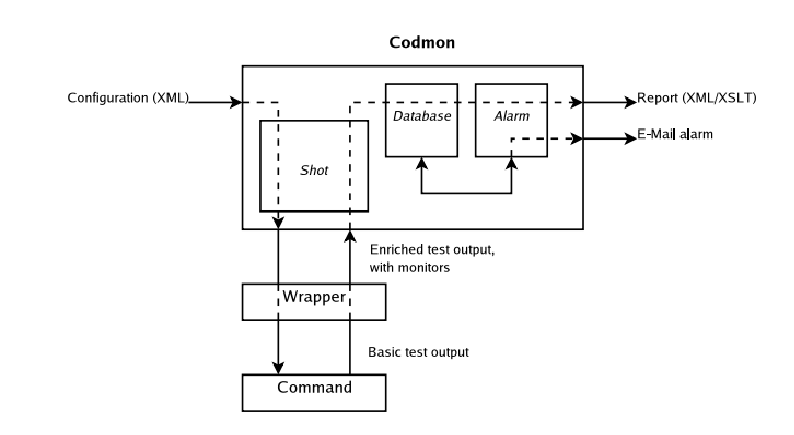
\includegraphics[scale=0.5]{codmon}
\end{figure}



\subsection{Codmon problems}
\label{subsec:CodmonProblems}
The goal of this research was to see if it's possible to design a multi-platform, user friendly modular test environment. There are multiple reasons why Codmon doesn't fit the bill. First,
to be multi-platform, without applying every change multiple times, the platform itself must be written in a platform-independent language. If we take a look at Codmon there are at least three 
different languages used. The core of Codmon is written in Java, which is indeed platform independent\cite{Java}, so this is not the real problem. As we've explained in section \ref{subsec:CodmonDesign} the
core-part of the sensors is a combination of a \emph{shell-script} command and a \emph{wrapper}. Since a Linux shell-script will usually won't work on a Windows environment this part is definitely
not platform independent. The same can be said about the PERL language, this will without special effort, also not work on a Windows environment. Next to this there are also several separate
scripts for example, for  CVS-checkouts and the startup of the Codmon framework. Taking this into account, we can easily see that the Codmon framework is far from platform independent. Due to the chaos of 
different scripts and languages it is also difficult for programmers to add new modules or tests to the Codmon framework. In the reminder of this thesis we'll explain how \project{} solves
these and other issues. 

\newpage
\section{The Road to \project{}}
\label{sec:road}

//TODO: Explain ideas and road to solution

\newpage
\section{The implementation of \project{}}
\label{sec:Codmon2.0}
//TODO: Section describes the implementation of the \project{} project.
\subsection{The init.XML file}
\label{subsec:init}

\subsection{Version control}
\label{subsec:versionControl}

\subsection{wrappers}
\label{subsec:wrappers}

\newpage
\section{evaluation}
\label{sec:evaluation}
TODO: This section evaluates the choices that are made in the previous sections'

\newpage
\section{Conclusion and related work}
\label{sec:conclusion}
TODO: give answers to the questions from section Problem statement
TODO: Discus related and future work
\newpage

\bibliography{Master}
\end{document}    